\adparagraph{nDCG}

\begin{figure}[H]
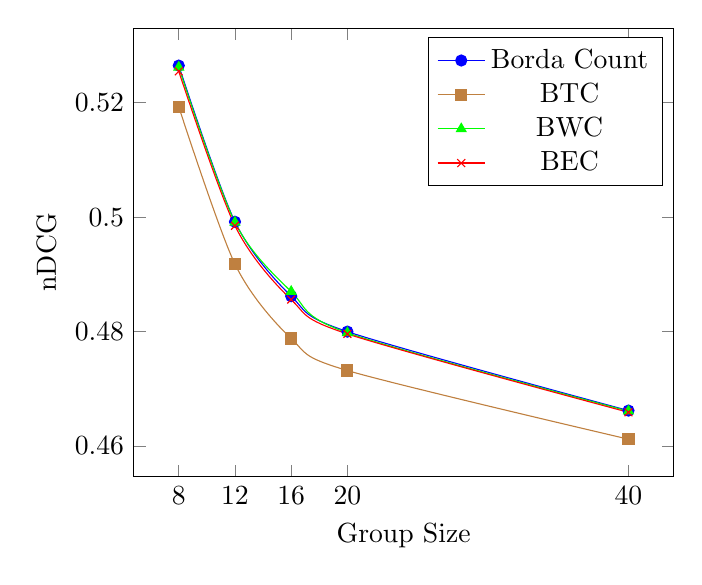
\begin{tikzpicture}
\begin{axis}[
	xlabel=Group Size,
	ylabel=nDCG,
	xtick = {4,8,12,16,20,40}]
		\addplot[smooth,mark=*,blue] plot coordinates {
		%(4,0.6028)
		(8,0.5265)
		(12,0.4992)
		(16,0.4862)
		(20,0.48)
		(40,0.4662)
	};
	\addlegendentry{Borda Count}
	
	\addplot[smooth,color=brown,mark=square*] plot coordinates {
		%(4,0.5995)
		(8,0.5193)
		(12,0.4918)
		(16,0.4788)
		(20,0.4732)
		(40,0.4612)
	};
	\addlegendentry{BTC}
	
	
	\addplot[smooth,color=green,mark=triangle*] plot coordinates {
		%(4,0.6022)
		(8,0.5262)
		(12,0.4991)
		(16,0.487)
		(20,0.4798)
		(40,0.4661)
	};
	\addlegendentry{BWC}
	
	
	\addplot[smooth,color=red,mark=x] plot coordinates {
		%(4,0.6010)
		(8,0.5255)
		(12,0.4985)
		(16,0.4856)
		(20,0.4796)
		(40,0.4659)
	};
	\addlegendentry{BEC}

\end{axis}
\end{tikzpicture}
\caption{Results on nDCG test on Borda Count extensions}
\end{figure}